\section{Simulation and Performance}\label{sec:performance}

The author compares the OBKF with the model specific Kalman filter, IBRKF, minimax Kalman filter, and MAP Kalman filter. The model specific Kalman filter is the classic KF with true unknown parameter. The minimax Kalman filter provides the best worst case performance. The MAP Kalman filter is the classic KF with the MAP estimates of the unknown parameter. 
To evaluate the estimation, the covariance of the estimation error is used. In the equation (\ref{eq:metric}), ${\bf P^x}_{k+1}(\bm{\theta};\bm{\theta}')$ is the covariance of the estimation error $\bm{x}_k-\bm{\hat x}_k$. 

\begin{align}\label{eq:metric}
{\bf P^x}_{k+1}(\bm{\theta};\bm{\theta}') &= \bm{\Phi}_k({\bf I}-{\bf K}^{\bm{\theta}'}_k{\bf H}_k){\bf P^x}_k(\bm{\theta};\bm{\theta}')({\bf I}-{\bf K}^{\bm{\theta}'}_k{\bf H}_k)^T\bm{\Phi}^T_k \nonumber \\
&\quad + \bm{\Gamma}_k{\bf Q}^{\theta_1}\bm{\Gamma}_k^T + \bm{\Phi}_k\bm{K}_k^{\bm{\theta}'}\bm{R}^{\theta_2}(\bm{K}_k^{\bm{\theta}'})^T\bm{\Phi}_k^T
\end{align}

The trace of ${\bf P^x}_{k+1}(\bm{\theta};\bm{\theta}')$ is computed as the MSE of the estimation, and it is used as the metric.

To evaluate the performance of the OBKF, consider a 2-D tracking problem with an unknown parameter. In the problem, the state vector is $\bm{x}_k=[p_x\, v_x\, p_y\, v_y]^T$, where $p_x,\, v_x,\, p_y,\, v_y$ are the position and velocity of the x and y dimmensions, respectively. The parameters in the (\ref{eq:linear1}) and (\ref{eq:linear2}) are given as follows.

\begin{align*}
    &\bm{\Phi}_k=
    \begin{bmatrix}
        1 & \tau & 0 & 0\\
        0 & 1 & 0 & 0 \\
        0 & 0 & 1 & \tau \\
        0 & 0 & 0 & 1 \\
    \end{bmatrix}, \;\;
    \bm{H}_k = 
    \begin{bmatrix}
        1&0&0&1\\
        0&0&1&0
    \end{bmatrix}, \;\;
    \bm{\Gamma}_k = \bm{I} \\
    &\bm{Q} = q \times 
    \begin{bmatrix}
        \tau^3/3 & \tau^2/2 & 0 & 0 \\
        \tau^2/2 & \tau & 0 & 0 \\
        0 & \tau & 0 & 0 \\
        0 & 0 & \tau^2/2 & \tau
    \end{bmatrix}, \;\;
    \bm{R}=r\times\begin{bmatrix}
        1&0\\
        0&1
    \end{bmatrix}
\end{align*}

Here, $\tau$ is the measurement interval. $q$ and $r$ are the covariance noise intensity.

In the simulation, the author uses $\tau = 1$ second. The initial conditions are set as $\E[\bm{x}_0]=[100\, 10\, 30\, -10]^T$ and ${\rm cov}[\bm{x}_0]={\rm diag}([25\, 2\, 25\, 2])$ where ${\rm diag}(v)$ is a diagonal matrix whose diagonal elements are $v$.
The parameter $q$ is set to 2 and $r$ is defined as a random variable, uniformly distributed over [0.25,4]. 

\begin{figure}[H]
    \begin{center}
    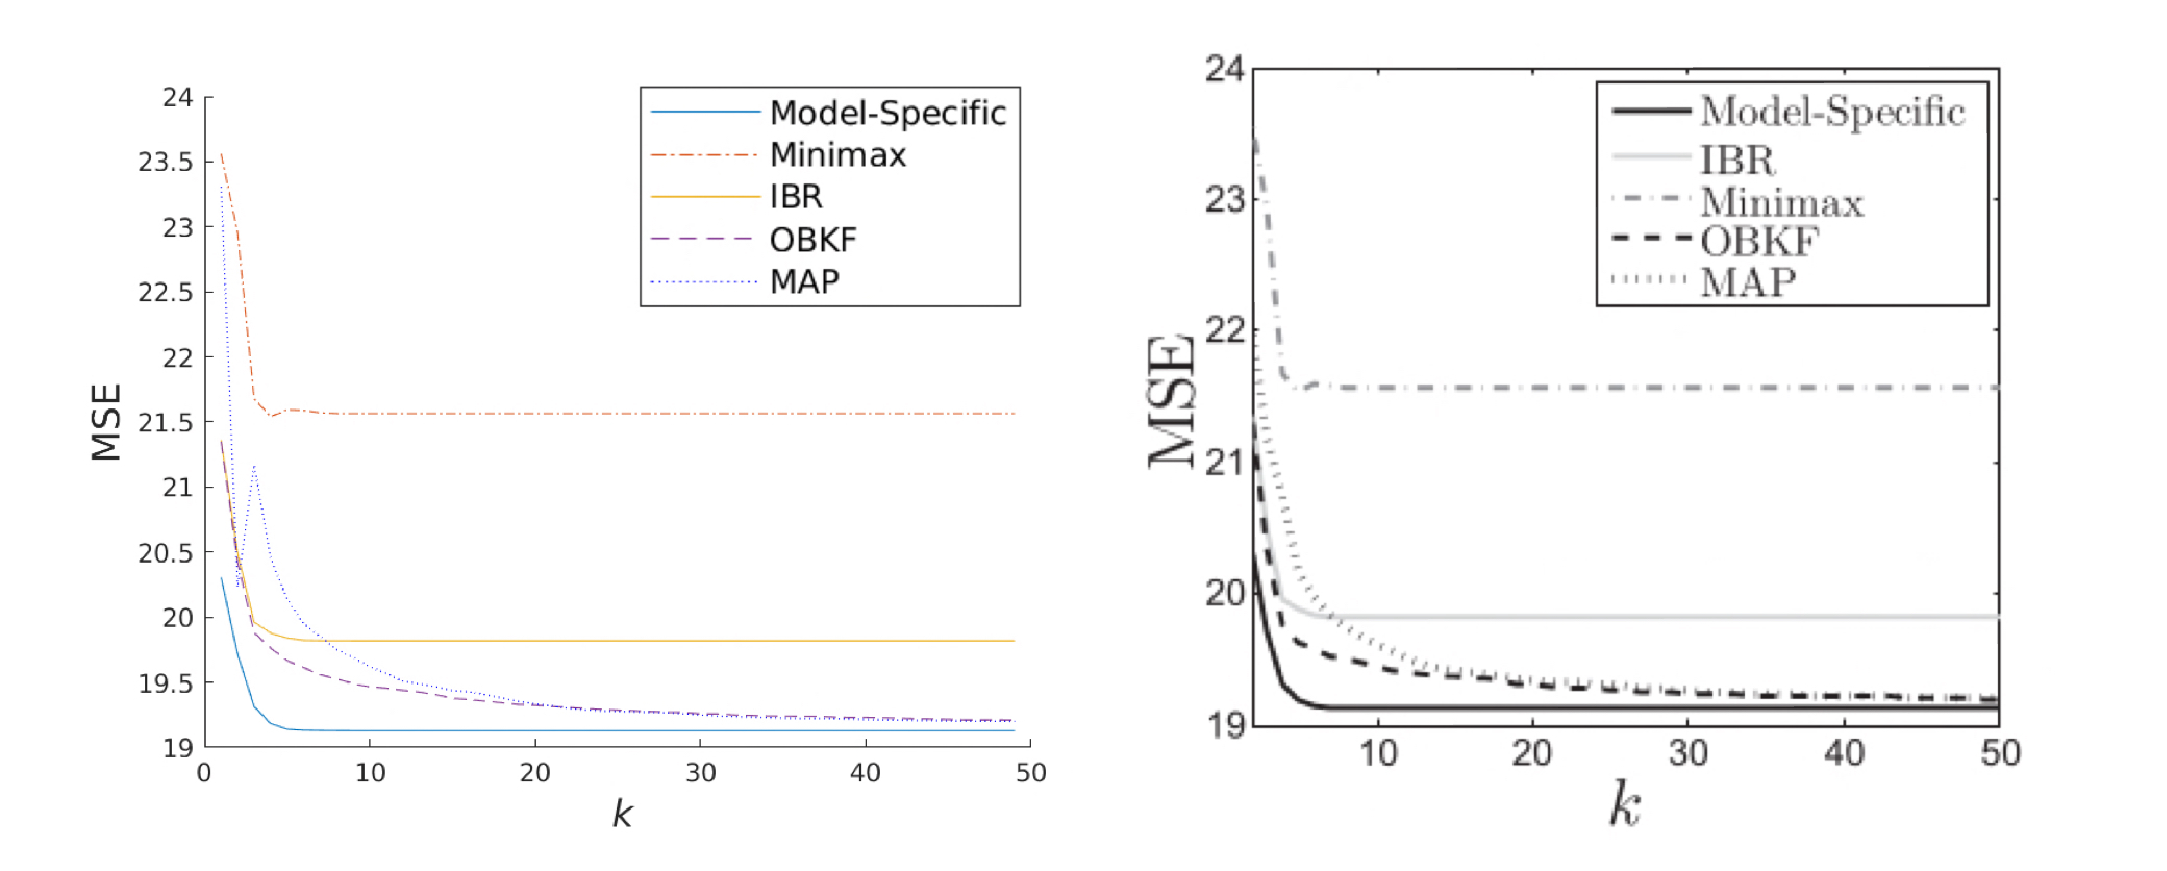
\includegraphics[width=9.7cm]{img/r1_mse.eps}
    \caption{MSE for $r=1$. The left figure shows the result simulated on my laptop. Right figure is cited from the OBKF paper\cite{Dehghannasiri2018}.}
    \label{fig:mse_r1}
    \end{center}
\end{figure}
\begin{figure}[H]
    \begin{center}
    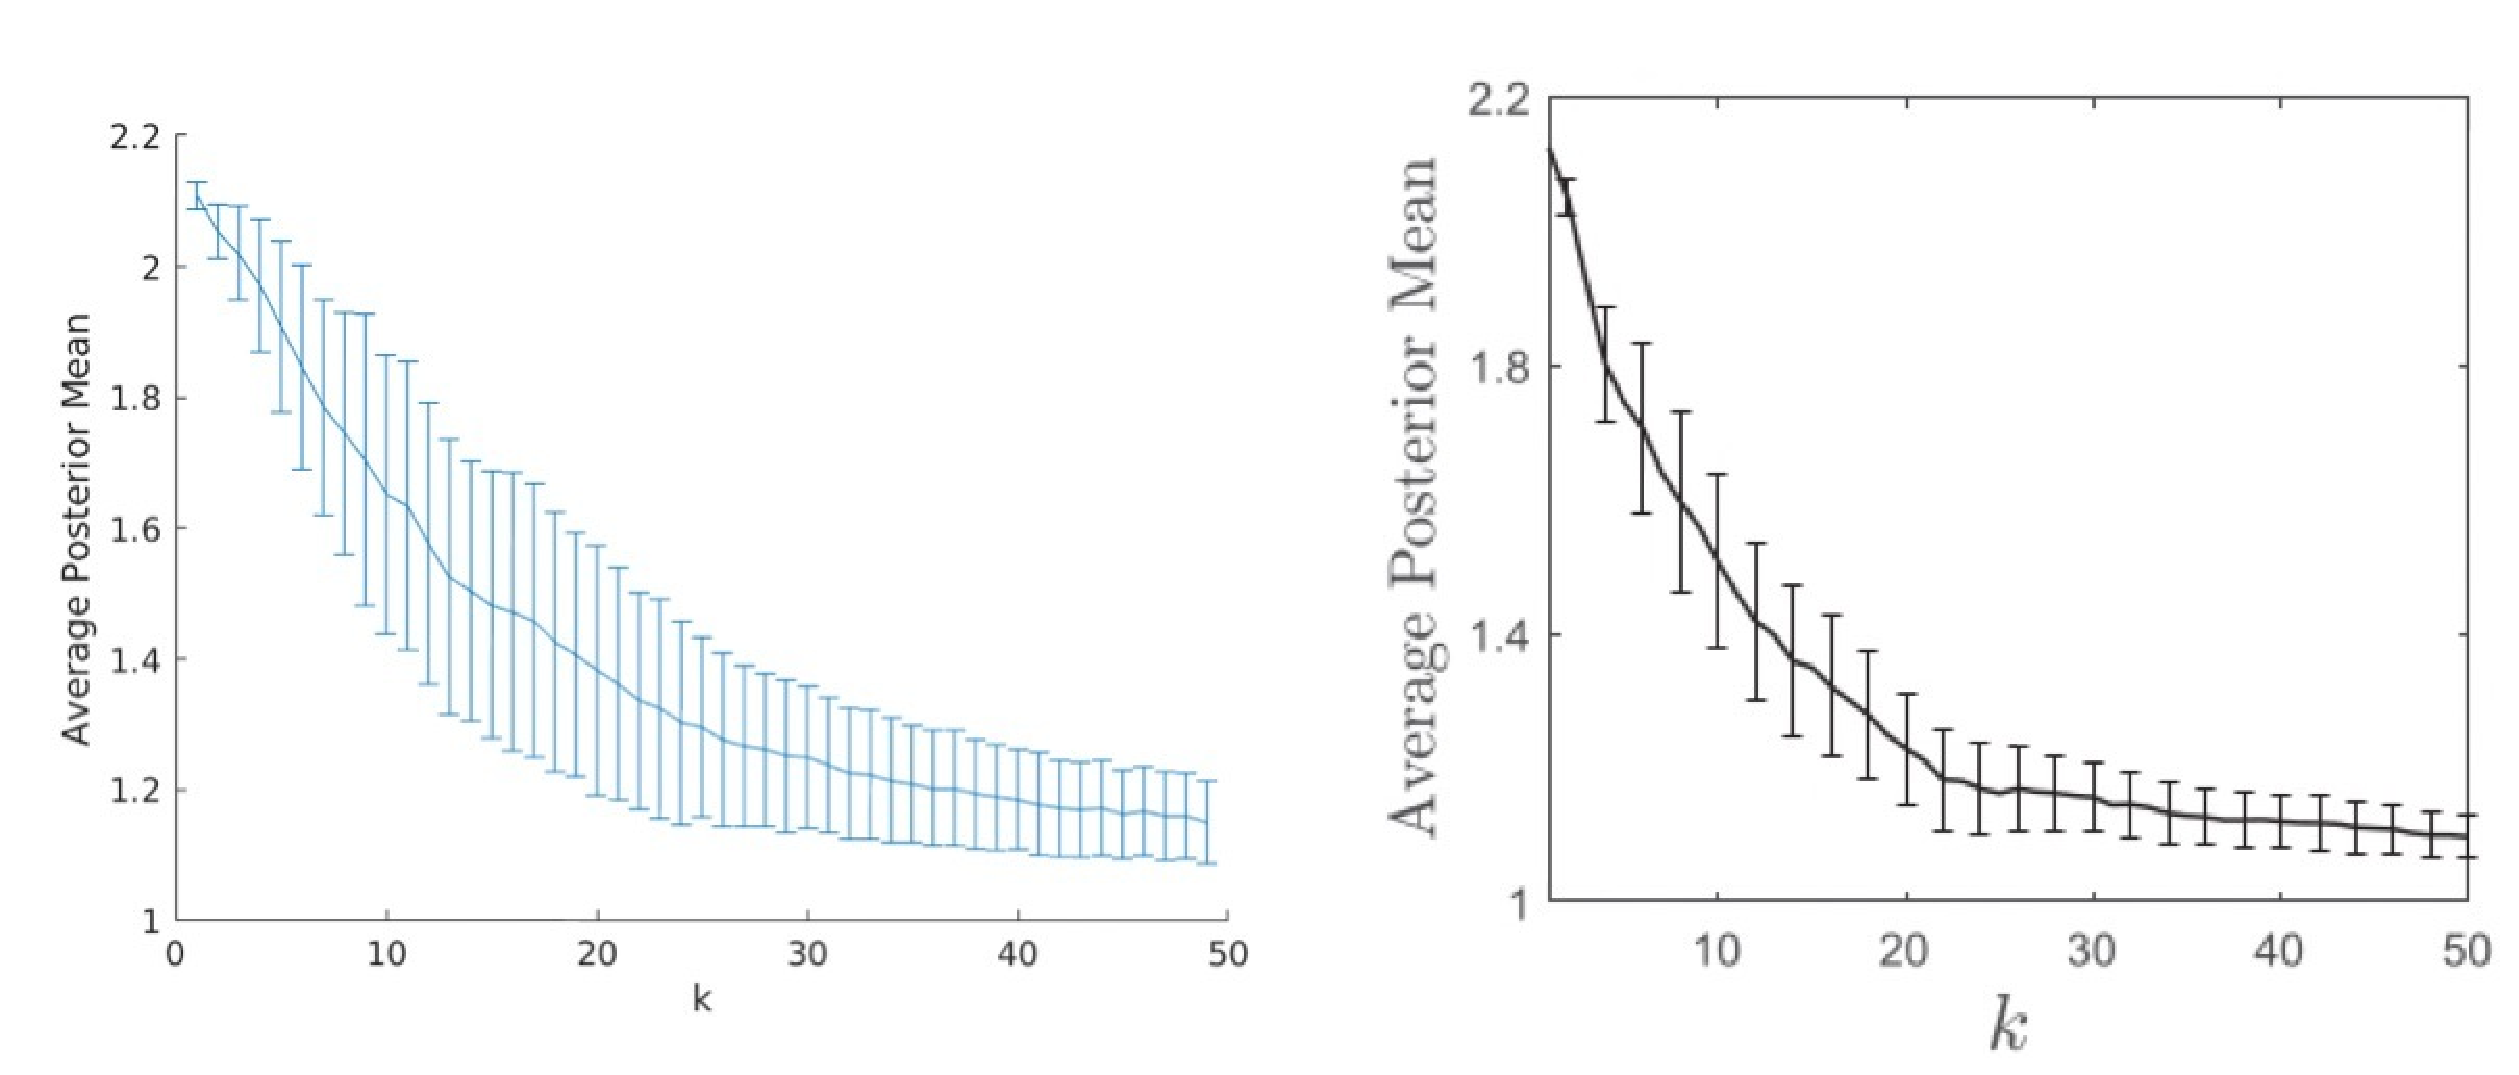
\includegraphics[width=9.7cm]{img/r1_mean.eps}
    \caption{Empirical average and variance of $\E[r|\mathcal{Y}_k]$. The left figure shows the result simulated on my laptop. Right figure is cited from the OBKF paper\cite{Dehghannasiri2018}.}
    \label{fig:mean_r1}
    \end{center}
\end{figure}

From the view of the estimation accuracy, the OBKF achieves the best performance. Fig.\ref{fig:mse_r1} compares the simulated MSE on my laptop with the figure from the paper. You can see that in the both images, the OBKF outperforms the other Kalman filters. The OBKF converges. The OBKF converges the fastest and reaches almost the model-specific KF as $k$ increases. Fig.\ref{fig:mean_r1} compares the estimated $r$ simulated on my laptop and the figure from the paper. In the both image, the estimated $r$ converges to the true value $r=1$ as k increases. That means that the estimation is getting close to the model-specific KF as the $k$ increases.

\begin{figure*}[h]
    \begin{center}
    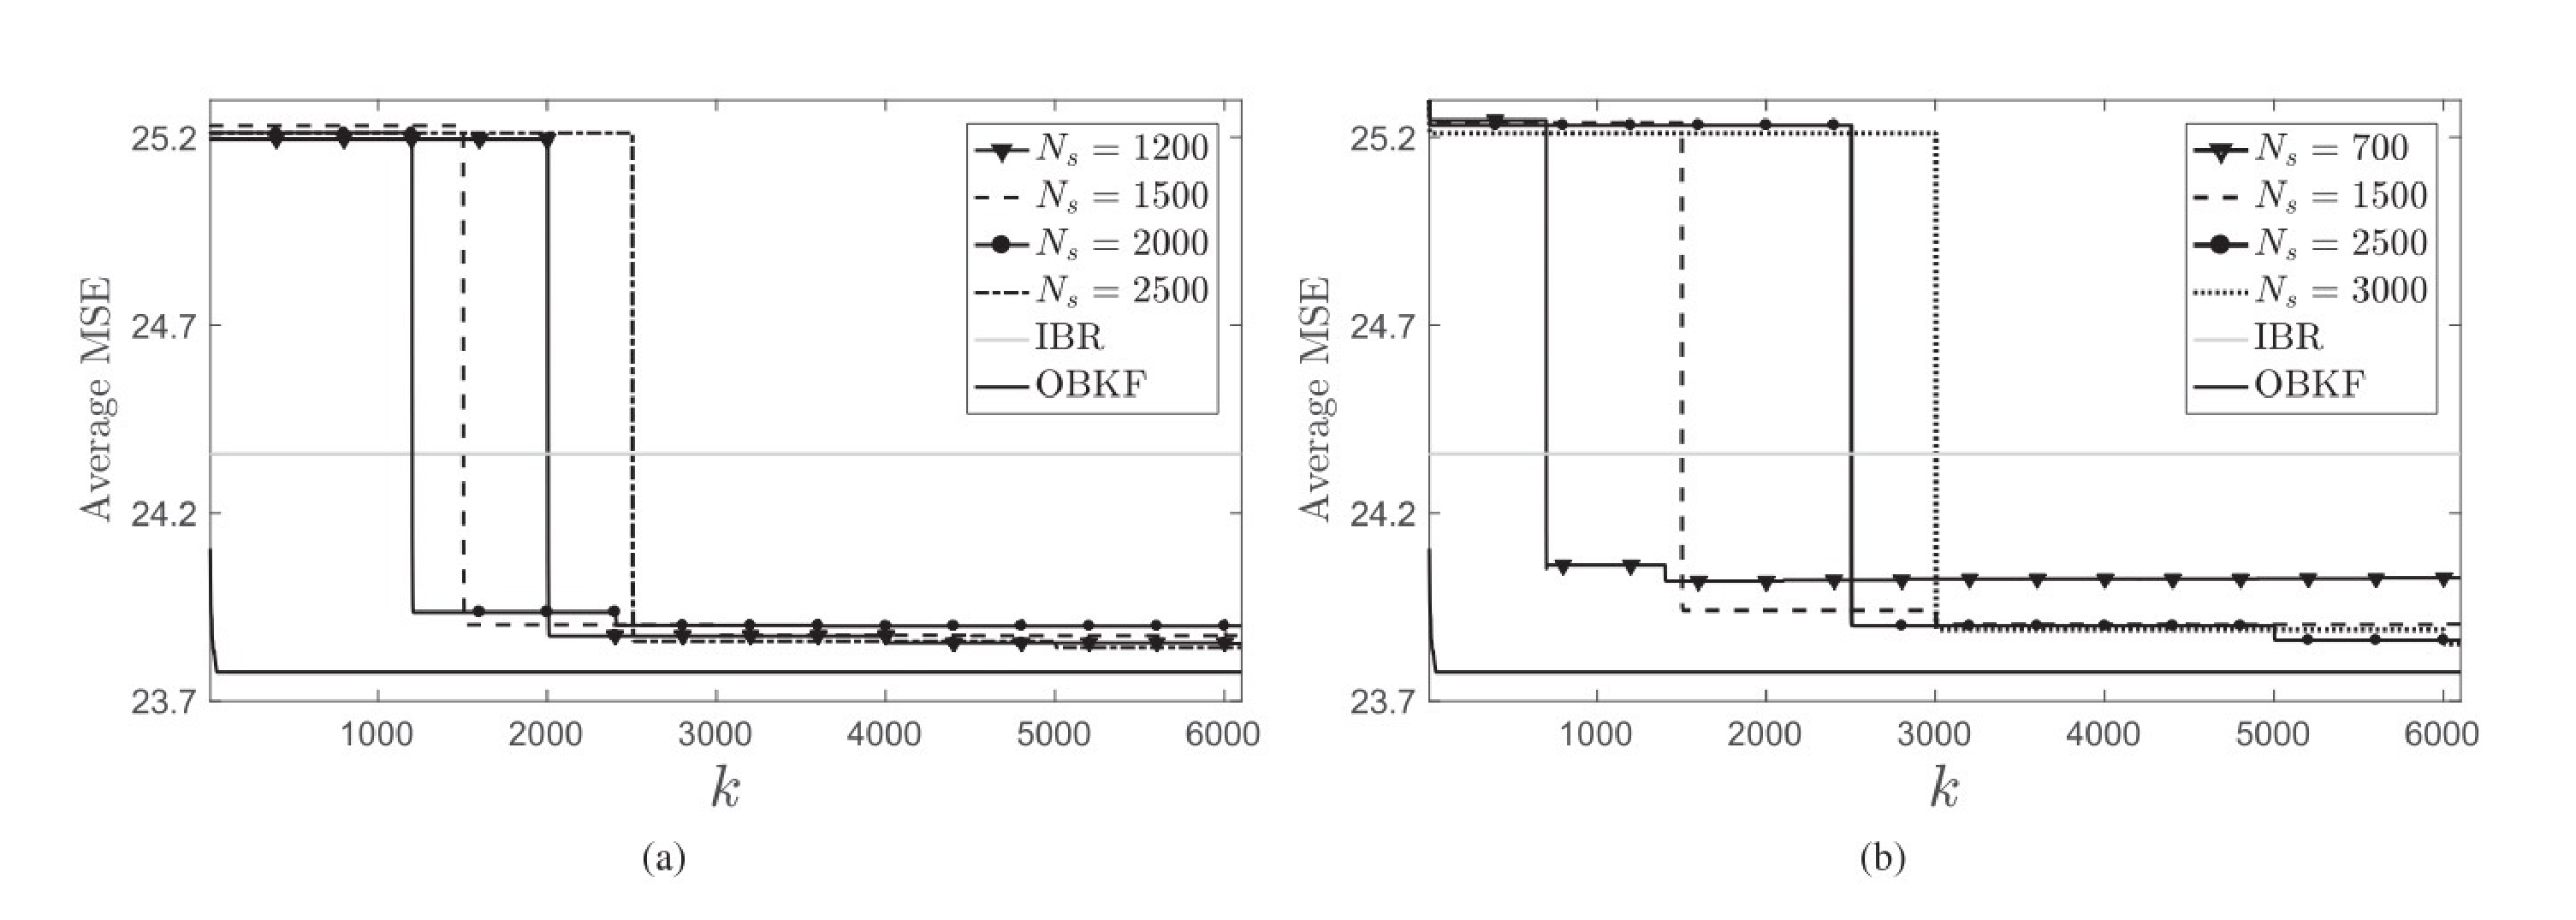
\includegraphics[width=15cm]{img/cmp_adaptive.eps}
    \caption{Comparison with the adaptive Kalman filters. (a) Unknown $r$ and comparison with the Myers method. (b) Unknown $r$ and comparison with the Mehra method. Cited from \cite{Dehghannasiri2018}}
    \label{fig:cmp_adaptive}
    \end{center}
\end{figure*}

Compared with the non-bayesian approach, the OBKF achieves much efficient estimation in the sense of the number of data. Fig.\ref{fig:cmp_adaptive} compares the OBKF and the adaptive Kalman filter with unknown parameter $r$ uniformly distributed over [0.25, 4]. The adaptive methods depend on the parameter $N_s$, which is the number of the observations to tune the filter. If the $N_s$ is small, the adaptive Kalamn filter estimates poorly and can be unstable in the long run. From Fig.\ref{fig:cmp_adaptive}, you can see that the OBKF converges much faster than the adaptive methods.

\begin{figure}[H]
    \begin{center}
    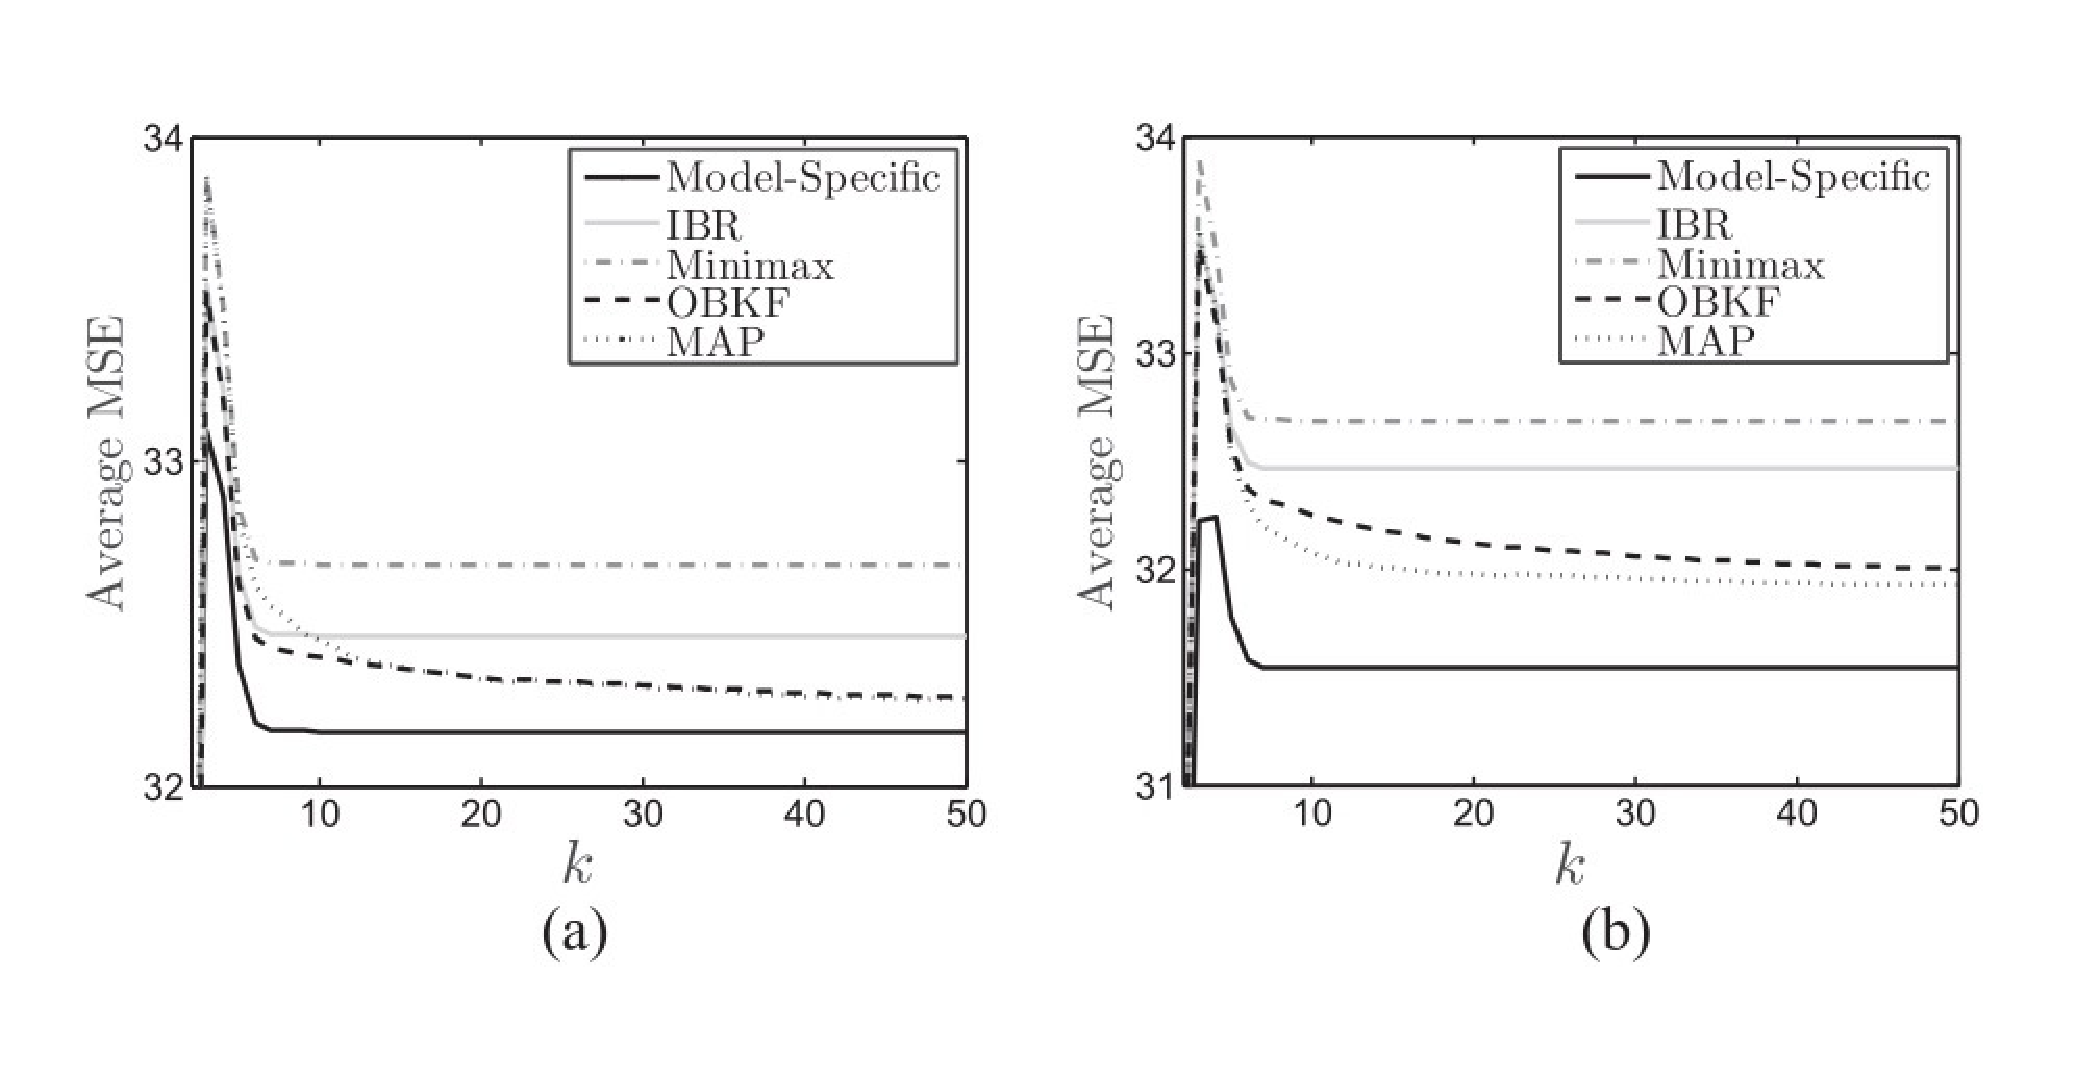
\includegraphics[width=10cm]{img/wrong_prior.eps}
    \caption{Average performance with unknown $r$. The assumed prior distribution is uniform distribution over the interval [3, 6]. (a) True uncertainty interval [2, 7] (b) True uncertainty interval [0.5, 8.5]. Cited from \cite{Dehghannasiri2018}}
    \label{fig:wrong_prior}
    \end{center}
\end{figure}

Although the OBKF is accurate and efficient, the accuracy of the OBKF depends on the prior knowledge. If the true prior distribution is different from the prior distribution in the OBKF, the OBKF doesn't converge to the optimal performance. Fig.\ref{fig:wrong_prior} shows the MSE of the Kalman filters with incorrect prior distribution. Since the prior distribution doesn't include the true value in some simulation, there is a possibility that the OBKF doesn't find the true value. 